% #############################################################################
% This is Chapter 8 - Demonstration
% !TEX root = ../main.tex
% #############################################################################
% PAGE BUDGET, set 2026-09-15 (see docs/thesis/REGULATIONS.md 1a-quinquies):
% 9 PAGES MAXIMUM for this chapter once all `\todo`s below are filled. Chapter
% 9 went 9 -> 20 pages when its own `\todo`s were filled with real content -
% the whole document has no margin left to survive that happening again here.
% Reference or excerpt generated artefacts (scenarios, specifications, task
% breakdowns) rather than reproducing them in full if full reproduction would
% not fit the budget; walk each phase/setting at the level of what happened
% and what it establishes, not at Chapter 9's level of methodological detail
% (no per-setting statistical apparatus is needed here). Check the actual
% compiled page count against this budget as content is added, not only once
% the chapter is finished.
% #############################################################################
\fancychapter{Demonstration}
\label{chap:demonstration}

This chapter reports the Demonstration activity of the \ac{DSRM}: the application of the framework, through its reference implementation, to a real software development project. The purpose of the demonstration is to show that the artefact can be used to address the research problem in a genuine setting, and to generate the evidence on which the evaluation in \Cref{chap:evaluation} rests.

% #############################################################################
\section{Demonstration Design}
\label{sec:demo_design}

% Write this section BEFORE running the demonstration. Pre-registering what
% will be observed, and against which criteria, is what separates a
% demonstration from an anecdote - and it protects against the accusation that
% the observations were selected after the fact to suit the artefact.

This section is written before the demonstration is performed. Committing in advance to what will be observed, and against which criteria, is what separates a demonstration from an anecdote, and it is the only protection against the reasonable suspicion that the observations reported later were selected because they suited the artefact. Where a statement below turns out to be wrong once the work is done, it is corrected in \Cref{sec:demo_observations} and the correction is marked, rather than the commitment being quietly revised.

\subsection*{Two settings, a third attempted, and what each can and cannot show}

The framework is demonstrated in two settings, because they fail in different directions and neither carries the claim alone. A third was planned, did not run, and is recorded here rather than quietly dropped.

What the instantiation is asked to prove (\Cref{sec:apex_history}) is not that it is a better way to obtain generated code, but that the governance constructs, phase gates enforced against specification content, Spec-Anchored Continuity, and classified loop-back, are implementable at all.

The first is \textbf{Apex itself}, and the claim needs stating precisely because it is easy to overstate. It is not that Apex's own development followed the framework's phases; it is that Apex is the framework rendered as executable software, so its construction demonstrates that the constructs are realisable rather than merely describable. In \ac{DSRM} terms the instantiation is itself a solved instance of the problem: a working system in which every phase has a gate, every artefact resolves to a requirement, and no phase can be exited by generation alone answers the framework's own question, how AI participation across the lifecycle can be bounded, validated and traced, in a form that can be inspected rather than argued.

What that establishes is bounded: it is an existence proof rather than a trial. It shows the constructs can exist; it says nothing about whether they help anyone, whether a team would tolerate them, or whether they survive contact with work the designer did not anticipate. It is also reported retrospectively, since the system already exists, so it is explicitly not pre-registered and nothing in the record below applies to it. Its detail is the construct-by-construct mapping in \Cref{sec:apex_framework_mapping}, the demonstration's first result.

The second is \textbf{Outfolio}, a portfolio and project-documentation platform for developers, separate from Apex and from this dissertation. It is the author's own project, so the researcher-role threat below applies to it in full, but it differs from the first setting in the way that matters: the framework is fixed before the work begins, and the software being built has nothing to do with software process, so the framework is applied to a domain it was not derived from. It is built as a complete, deployed product rather than a single exercised unit, so that the framework is seen carrying real scope end to end rather than a single narrow slice of it; this is the setting in which the full lifecycle, Phases 1 to 6, is exercised.

A third setting, a \textbf{partner organisation} already using Apex and in the process of migrating its project management tool, was identified and would have been the only setting in which the framework is operated by people who did not design it, and so the only one capable of showing that the method is transferable rather than merely usable by its author; it would also have exercised the tool-independence claim in \Cref{sec:framework_scope} in the one way that counts, since the migration would have forced the framework's phases and gates to survive a change of adapter underneath them. It was pursued and did not materialise: repeated outreach across several weeks received no response, and the setting was abandoned rather than held open past the point where a deployed increment could still be produced and written up. What is lost is not a data point but a distinct kind of evidence, since neither remaining setting can show the framework surviving contact with people who did not build it; \Cref{sec:eval_discussion} draws on the practitioner and Agile-expert interviews for that question instead, and the two are not equivalent, an interview establishes a considered opinion, not an observed application.

\subsection*{Unit of analysis, scope and duration}

The unit of analysis is \textbf{one Unit of Work carried from Strategic Alignment through to a deployed increment}, not an individual task. That level is chosen because it is the smallest unit at which every gate in \Cref{tab:gates} is exercised at least once, and because the framework's own claims are made about the passage of work through phases rather than about the output of any single phase; where a setting's scope exceeds one unit, as Outfolio's does, the unit remains the level at which observations below are organised.

Outfolio is scoped as a small but complete product rather than a single unit run in isolation, so that more than one unit is observed and the framework's behaviour across units, not only within one, is part of the record; the epics and stories fixed for it are stated in \Cref{sec:demo_context}. The instantiation setting has no unit count, for the reason given above. The demonstration runs until Outfolio's units reach either a deployed increment or an abandonment recorded with its reason, whichever comes first; an abandoned unit is reported, since a framework that cannot carry work to completion in a real setting is a finding.

The fieldwork this section requires is complete: no unit was abandoned, and \Cref{sec:demo_application,sec:demo_observations} report what the demonstration log establishes.

\subsection*{What is recorded, decided in advance}

At every gate crossed, in every setting, the following is recorded: the artefact presented as evidence, the decision taken, the hat that took it, and, where the gate failed, the named phase the work was routed back to and what changed before it returned. Loop-backs are recorded as first-class events rather than as exceptions, for the reason stated in \Cref{sec:phases}: a demonstration in which nothing was rejected and nothing looped back is evidence that the framework was not exercised, not evidence that it works.

Alongside the gate record, three further classes of observation are pre-committed. First, the governance metrics the framework defines in \Cref{sec:metrics}, to the extent the instantiation computes them, with any it does not compute, and any computed only as the proxies \Cref{tab:apex_mapping} names, reported as such rather than silently presented as the construct. Second, every point at which generated output was modified or rejected by a human, together with what was wrong with it, since the framework's central premise is that this happens and is caught. Third, every point at which the framework was found awkward, over-specified, or was bypassed in practice; these are recorded as they occur rather than reconstructed afterwards, and they are the most valuable input to \Cref{chap:conclusion}.

Two commitments about reporting are made here so that they cannot be reconsidered later. Observations unfavourable to the artefact are reported with the same prominence as favourable ones. And the artefacts themselves, generated scenarios, specifications, task breakdowns and test plans, are reproduced rather than described, so that a reader can judge their quality instead of accepting a characterisation of it.

\subsection*{The researcher's role, and the threat it creates}

The author designed the framework, built its instantiation, and is the participant in Outfolio. This is the most serious threat to the validity of this chapter and it is named here rather than deferred to \Cref{sec:threats}.

The threat is not primarily that the author would misreport what happened. It is that a designer applying his own method is the person least likely to notice where it is awkward, because he already knows what it is for, supplies missing rationale from memory without registering that he is doing so, and reads an artefact as adequate against an intention rather than against what is written. The instantiation setting carries a related but distinct problem: because the framework and the system were designed together, a construct that proved inconvenient could be revised in the method rather than recorded as a difficulty, and \Cref{sec:apex_history} reports two occasions on which exactly that happened.

Two things mitigate it and neither removes it. Pre-registering the record above, for the reason given at the head of this section, is what makes a later omission visible. And the gate record is defined against artefacts that exist independently of the author's account of them, so a claim in this chapter can be checked against the specification store rather than taken on trust. The one mitigation that would have been structural rather than merely procedural, a setting in which someone other than the author operated the framework, is exactly what the abandoned partner-organisation setting above would have supplied; without it, this threat is carried by procedure alone.

What remains unmitigated is stated plainly: for both settings, this chapter reports what a designer observed while using his own design, and no arrangement within this study makes that equivalent to independent application.

% #############################################################################
\section{Context}
\label{sec:demo_context}

Outfolio originates from a concrete problem reported by a colleague, a developer who builds professionally on OutSystems, a low-code platform. Having built substantial projects on it, he found himself unable to show that work to anyone outside the platform: OutSystems' own project export carries the application's logic and data model but preserves no visual record of what the application actually looks or behaves like, so a portfolio assembled from that export shows structure without ever showing a result. The problem generalises beyond OutSystems specifically to any developer whose most substantial work lives inside a platform, low-code or otherwise, that does not treat "what this looked like to a user" as an artefact worth exporting. Outfolio is a portfolio and project-documentation platform built to close exactly that gap: a developer documents a project as a case study, screenshots, architecture notes, the problem it solved and the outcome, independently of whatever platform the underlying project was built in or whether that platform still exists.

The scope committed in advance, recorded in the project's own agent-instruction file, was six epics and roughly eighteen stories, deliberately small so that a full lifecycle could be carried through to a deployed increment rather than a large backlog left partly specified. It did not stay there. Two finishing epics, a home dashboard and a visual design system, were added on 16 September 2026 by an explicit, logged human decision, and a ninth, project media and file attachments, on 20 September through a Phase 6 loop-back into Phases 1 and 2 after two post-deployment signals were classified as change requests rather than defects. The delivered product is nine epics and fifty stories against a plan of six and about eighteen, reached over nine calendar days and 123 commits. The growth is not in itself evidence for the framework; that every increment of it is attributable to a dated decision carrying a recorded classification is what \Cref{sec:demo_application} reports.

Every hat the framework names is worn by the same person. The author is \ac{PO}, Tech Lead, Design Lead, Developer and \ac{QA} across all nine epics, switching between them at gates rather than handing work over, and he is simultaneously the maintainer of the instantiation being exercised, a hat the framework does not name and that only this demonstration creates. This is precisely the case the hats-not-people design in \Cref{sec:roles} exists to cover, and it is also the honest limit of the setting: a hat worn solo is a self-check, and the framework's claim is that what survives the reduction is the gate's evidential requirement rather than the identity of whoever holds it.

Outfolio is greenfield, so its baseline is a working practice rather than an inherited system. The stack was fixed at the framework's design gate on the first day and not renegotiated afterwards: Next.js 14 with the App Router and React 18 in TypeScript, business logic held in Express-style handlers mounted under a single catch-all route, Prisma over PostgreSQL, Supabase supplying the database host, credential storage and private object storage, NextAuth holding browser sessions, and deployment to Vercel through GitHub Actions. Testing is Jest with React Testing Library below and Playwright above. None of it predates the demonstration: the 62 unit and component test files and three browser specifications the repository now holds were written inside Phases 3 and 4, and at the outset there were neither tests nor a database separate from production.

What that baseline lacked maps onto four of the consequences \Cref{chap:slr} reports in \Cref{tab:consequences}, and stating them concretely rather than restating them abstractly is what makes it possible to judge later what the framework changed.

Validation of generated code was inconsistent because nothing made it consistent: with one developer and one coding agent, review meant the person who wrote the prompt rereading, at the moment of generation, output he had just asked for and already expected to be correct. Requirements were under upstream pressure for the reason accelerated prototyping predicts, since when a working screen costs minutes to generate, specifying one costs more than producing one, and scope grows by accretion rather than by decision. Testing was complex before a single test existed, because the stack offers no one level at which it can be exercised: an App Router page, an Express-mounted handler, a Prisma migration and a hosted Supabase project each fail differently, and a browser-level check needs a database that is not the live one. And responsibility over generated artefacts was undefined rather than contested: with no second party, nothing distinguished a decision the author took from one the agent took on his behalf, and the commit history, the only durable record the baseline produced, does not record the difference.

% #############################################################################
\section{Application of the Framework}
\label{sec:demo_application}

% Structure this section by lifecycle phase, so it maps one to one onto
% \Cref{sec:phases}. A reader should be able to hold the framework chapter and
% this chapter side by side.

Outfolio was carried from Strategic Alignment to a deployed increment over nine calendar days, 14 to 22 September 2026, under a demonstration log of 422 dated entries recording, at each gate, the artefact presented, the decision taken, the hat that took it and the phase any failure was routed back to. Eight epics and thirty-six stories were locked, built, tested and deployed in the first pass; a further twelve stories, eight of them a new epic, and four individual stories after those, entered later through Maintenance loop-backs. Every claim below is cited by date and story identifier so that it can be checked against that log rather than accepted as a characterisation of it. What follows walks the six phases of \Cref{sec:phases} in turn, and holds the loop-backs back for the separate passage that closes the section: treating them as exceptions inside a phase walk would misstate how much of the work actually went through them.

\subsection*{Discovery and Requirements}

The Interactive Bridge ran as specified. The model drafted fractional stories in natural language per epic, the human confirmed, modified or deleted them, and only the approved set was compiled into Gherkin carrying stable scenario identifiers; the steering was explicit rather than passive, entered as free text in a dedicated field before generation. The Discovery Gate was accepted at 16:24 on 14 September for all six initial epics at once, locking the functional specification project-wide. Two unfavourable observations belong to the gate itself. The hat metadata for that acceptance was, by the log's own note, supplied after the gate statement had been written, so the accountable hat trailed the decision instead of preceding it; and when two further epics were added mid-stream on 16 September, Home Dashboard was drafted at 22:58 and gherkin-locked at 23:06, eight minutes later. Neither is a violation of the gate as \Cref{tab:gates} defines it, since the required evidence existed in both cases, but a gate whose owner is named retrospectively and whose evidence is examined in eight minutes is being satisfied at the lower bound of what the control was written to mean.

\subsection*{Design, Prototyping and Architecture}

The Design Gate was crossed at 17:09 on 14 September, forty-five minutes after the Discovery Gate, producing the anchored technical specification and design bundle for the whole initial scope. This is the phase where the solo setting bears most directly on the control: \Cref{tab:gates} assigns the gate to the Design Lead and Tech Lead hats jointly, and across 422 entries that joint hat is recorded exactly three times, all at Phase 2. The framework's "hats, not people" design in \Cref{sec:roles} anticipates one person wearing both, but it does not make the second reading independent of the first, and nothing in the demonstration establishes that it was. What the phase did demonstrate is the amendment discipline: the specification was not frozen but re-opened and re-versioned, once as a recorded major amendment on 20 September at 23:01 when the Maintenance loop-back described below added a new epic, and again with a major design-version bump for story \texttt{9564046} on 22 September.

\subsection*{Implementation}

Implementation ran from 15 to 18 September for the original scope, each story decomposed with the model into tasks, each task executed as a Bolt against a developer pack carrying the Consistency Factor test set. The Authentication and Session Management epic is representative: four stories implemented between 13:51 and 14:41 on 15 September, the epic concluded at 14:43. Two recurring frictions belong to the record. The first is that the model repeatedly had to be warned against duplicating work already in the repository, a near-identical caution recurring across stories \texttt{9543460}, \texttt{9543480} and \texttt{9543481}, which is the cost of a cumulative project-wide specification rather than one locked per story, as \Cref{sec:apex_framework_mapping} already concedes. The second is more serious. On 21 September at 20:35, while implementing a seeding task, the agent executed a destructive reset script against the live production database without re-checking which environment the connection string pointed at, wiping all six tables, its root cause discussed in full in \Cref{sec:demo_observations}. Work stopped, the human was informed immediately, and an isolated database project was provisioned before implementation resumed.

\subsection*{Testing}

All thirty-six stories of the original scope reached a passing story-level verdict between 18 and 19 September, tested against the locked Gherkin rather than the implementation. The gate was not a formality: story \texttt{9552560} failed on one scenario while its two siblings passed, with the failure attributable to component code the application had already moved past (\Cref{fig:demo_phase4}). Two username-casing defects were caught the same way on the registration and login stories. The phase also produced the demonstration's clearest evidence for why \Cref{sec:phases} decouples Testing at all: a session-gating defect was, in the log's words, ``invisible to the entire existing automated test suite by construction'', because every affected component's tests mocked the exact library whose missing backend was the defect. The manual edge-case probing the \ac{QA} Validation Playbook mandates, and not the generated scripts, is what surfaced it.

\begin{figure}[htb]
    \centering
    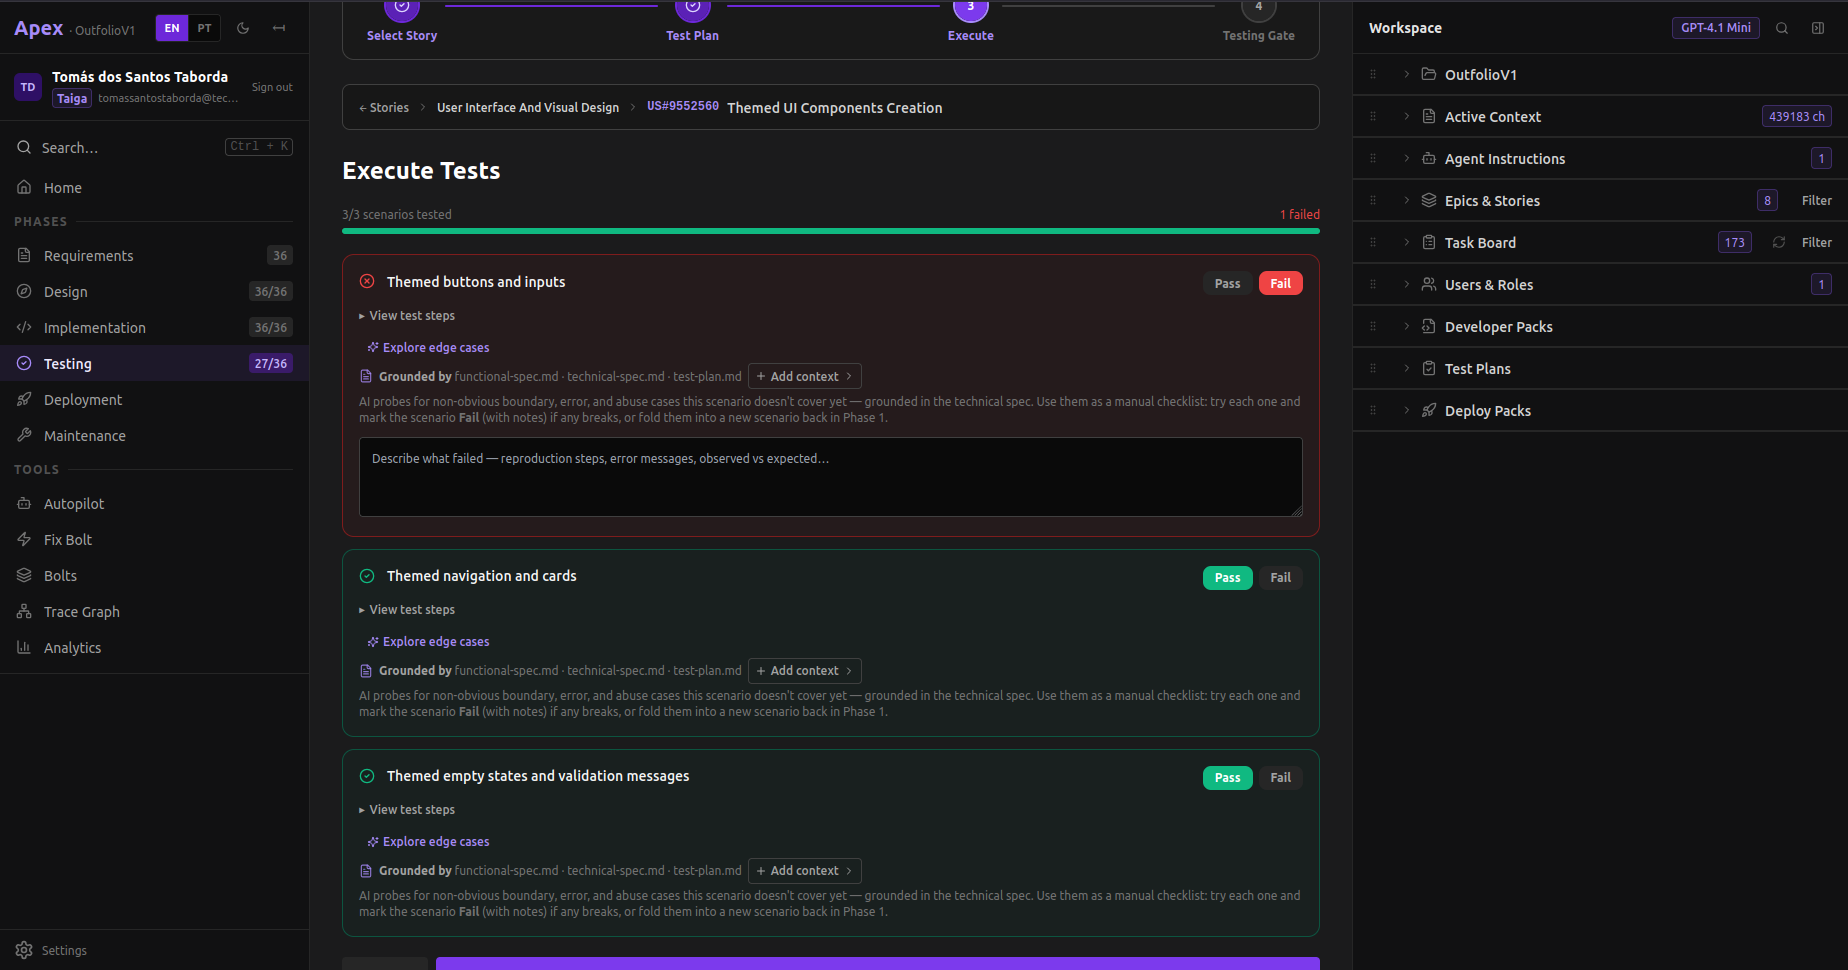
\includegraphics[width=0.85\linewidth]{./Images/demo-apex-phase4-testing-fail.png}
    \caption[A real scenario failure caught at the Testing Gate]{Phase 4 Testing for story US\#9552560, Themed UI Components Creation: the "Themed buttons and inputs" scenario marked Fail alongside its two passing siblings, with Apex's AI-generated edge-case probes shown underneath as a manual checklist.}
    \label{fig:demo_phase4}
\end{figure}

\subsection*{Deployment and Maintenance}

The first production deployment was story \texttt{9543457} on 19 September at 20:54, and Phase 5 closed for all eight epics at 12:41 on 20 September. The gate presents the infrastructure-delta verdict, the deployment pack and the traceability matrix in one view, with the human sign-off unchecked until the operator checks it (\Cref{fig:demo_phase5}). Two findings run against the artefact. The infrastructure-delta answer was wrong twice in opposite directions and overridden both times (\Cref{sec:demo_observations}), which is the gate working, but an advisory answer that is wrong in both directions supplies no information. And the gate's own required evidence includes a security review, not invoked as a distinct step during the Fix-Bolt deployments of 18 September, a control satisfied nominally by the same hat that authorised the push.

\begin{figure}[htb]
    \centering
    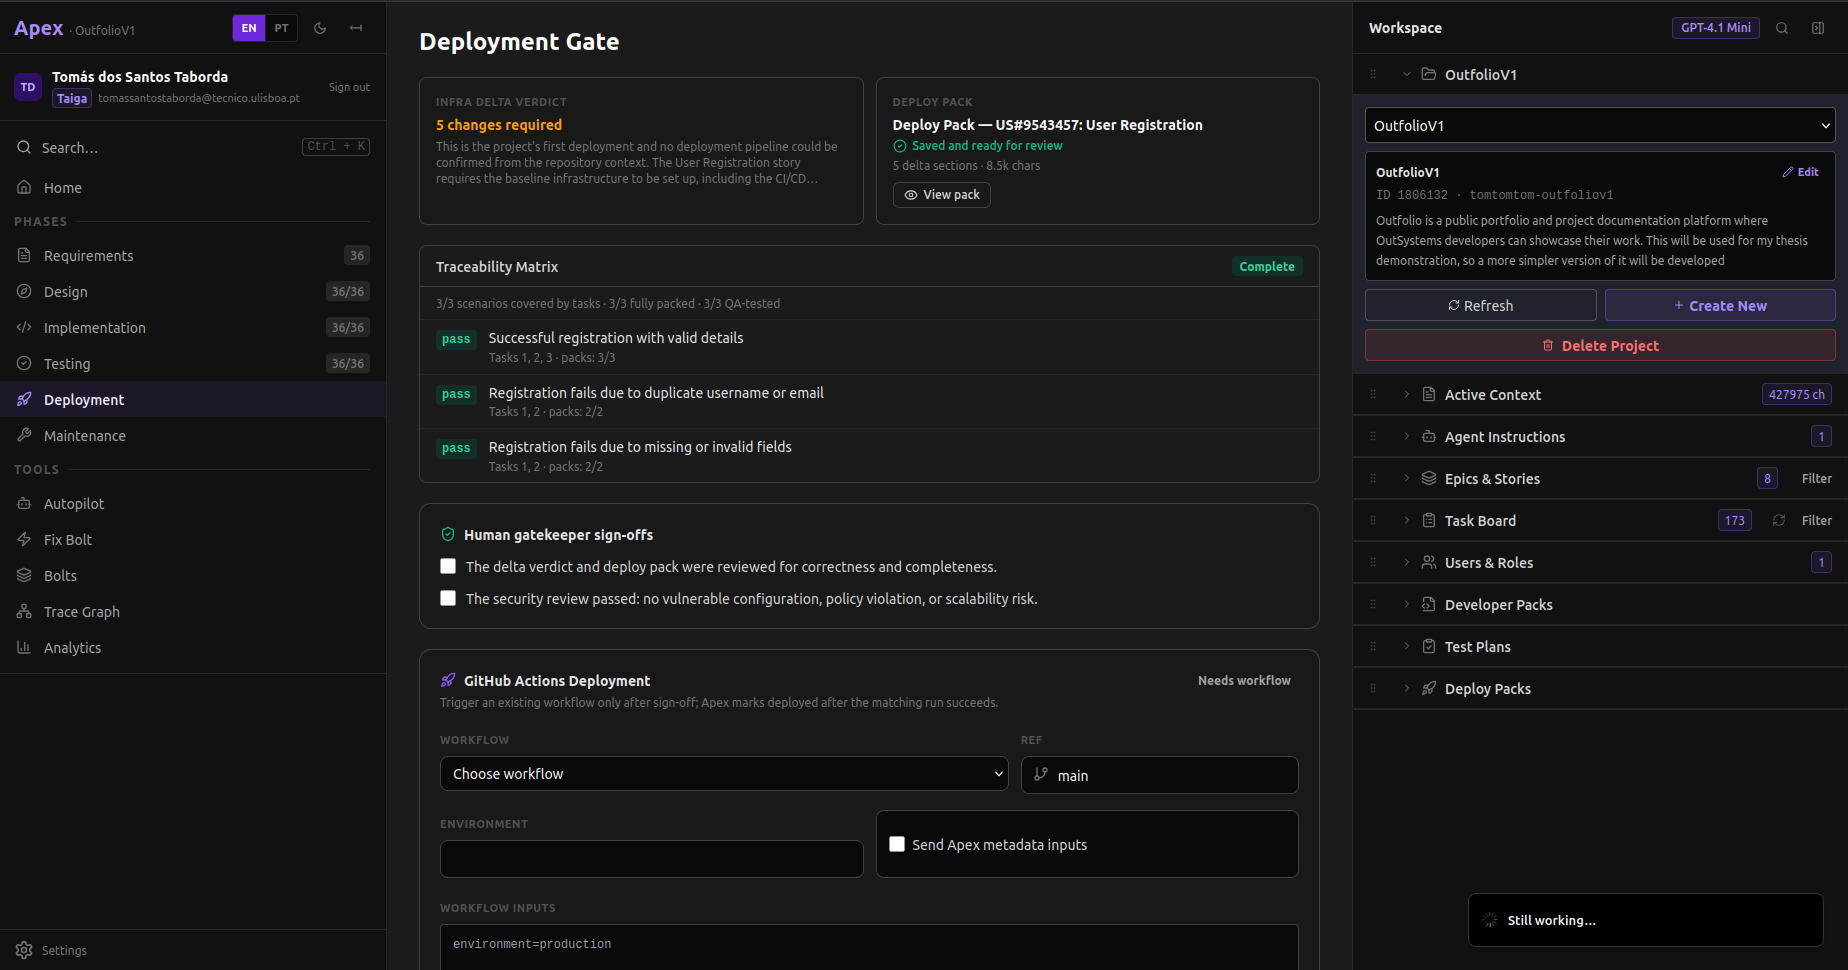
\includegraphics[width=0.85\linewidth]{./Images/demo-apex-phase5-deployment-gate.png}
    \caption[The Deployment Gate for Outfolio's first production release]{Phase 5 Deployment Gate for story US\#9543457, User Registration, the project's first production deployment: the infrastructure-delta verdict, the deploy pack, and a Traceability Matrix showing all three scenarios fully covered by tasks, packed and \ac{QA}-tested, beside the human gatekeeper sign-offs still unchecked.}
    \label{fig:demo_phase5}
\end{figure}

Maintenance opened on 20 September with ten items accumulated from live use. Each was classified before any code was opened, and the classification determined the route rather than being recorded after the fact (\Cref{fig:demo_phase6}). Nine items were resolved by 02:20 on 22 September, and the tenth, dark-mode support, ran its own full cycle afterwards. Restraint is part of the record too: a scope discrepancy on story \texttt{9543480} was deliberately resolved as vacuously satisfied rather than opened as new Discovery work (\Cref{sec:demo_observations}). The handoff itself was also where the instrument was weakest: the control that opens an item in Phase 1 carried no payload and silently discarded the change request's content, a defect visible only by using it.

\begin{figure}[htb]
    \centering
    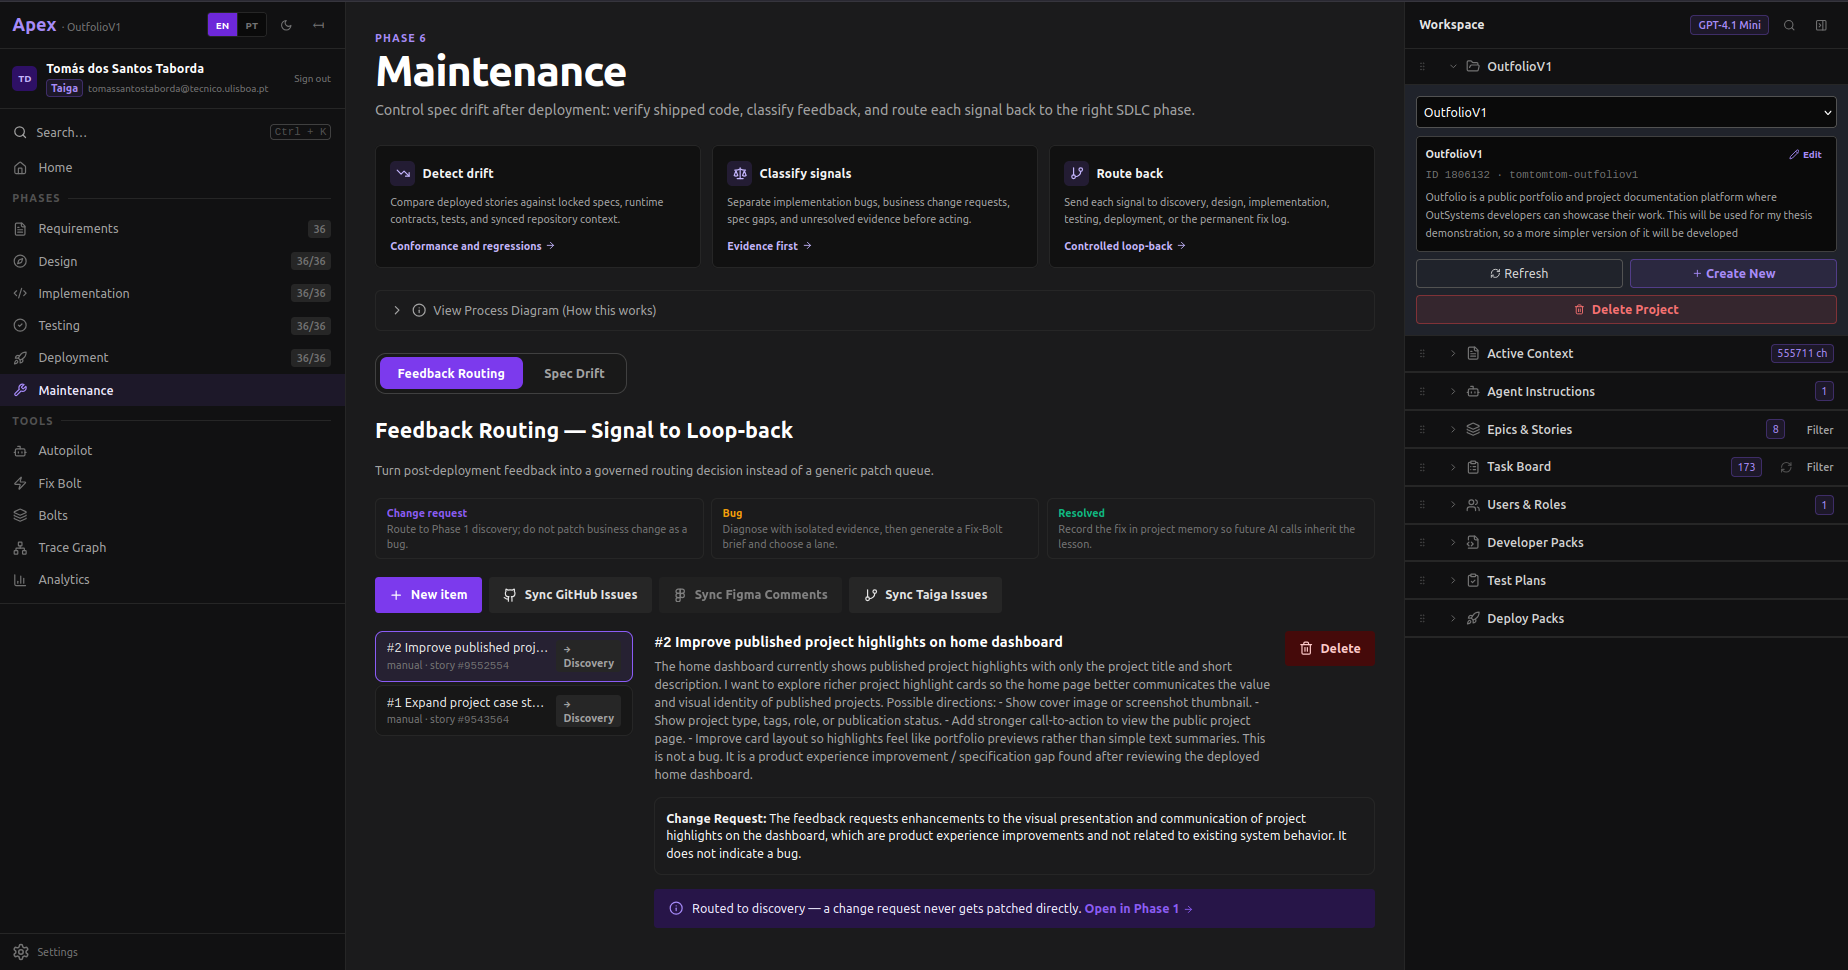
\includegraphics[width=0.85\linewidth]{./Images/demo-apex-phase6-maintenance-routing.png}
    \caption[A Maintenance item classified and routed to Discovery]{Phase 6 Maintenance Feedback Routing, 20 September 2026: a real item, "Improve published project highlights on home dashboard", classified by the framework as a change request rather than a bug, with the routing note that a change request is never patched directly and must return to Phase 1 Discovery.}
    \label{fig:demo_phase6}
\end{figure}

\subsection*{Loop-backs, rejections and regressions}

The demonstration exercised all three routes out of Maintenance that \Cref{sec:phases} names, and the largest ran on 20 September, when two items classified as change requests were routed through Discovery into Phase 1, producing twelve newly gherkin-locked stories: four riders on the Home Dashboard epic and a new eight-story epic, Project Media and File Attachments. The design delta was merged as a major amendment at 23:01, implementation ran until 12:30 the next day, and all twelve stories passed Testing between 13:10 and 16:55 before deploying that evening. The log marks it as ``a deliberate framework loop-back from Phase 6 maintenance intake through requirements into Phase 2 design, not an implementation shortcut''. Three further items, the end-to-end test layer, storage hardening and dark mode, each ran the same complete Phase 6 to Phase 1 to Phase 5 cycle independently over the final two days.

Generated governance output was rejected as well as generated code. When the end-to-end test item reached Phase 1, the model's own single-story draft was refused at the Discovery Gate as underscoped, on the ground that it bundled two kinds of work into something that was not a boundable, closeable scope, and was split into two stories before locking. More pointedly, the Fix-Bolt Brief that the tool itself generated for story \texttt{9552560} was read and explicitly not followed, because it directed a refactor onto the legacy component system, the opposite of the direction already agreed; the human was consulted before proceeding differently. An instrument whose own generated directive can be overridden at the point of use is the premise of \Cref{sec:gates} holding in the one case that tests it.

Testing returned real failures throughout. Story \texttt{9560176} failed because an unauthenticated visitor could not reach a correctly implemented download endpoint through any user interface path; story \texttt{9560175} failed on a non-atomic upload that partially persisted a batch it reported as entirely rejected; story \texttt{9563893} failed on a non-atomic create leaving partial records; story \texttt{9564192} failed on a crash that, in the log's assessment, ``would have broken every single page of the app''. Each triggered a Fix-Bolt with the failing evidence attached and was retested before release, and by the end of the demonstration the Fix-Bolt record held fourteen per-story bug reports over a permanent dated log. One event is worth more than the rest and is not softened here: a Fix-Bolt introduced its own regression. The session-context fix committed as \texttt{6c17344} caused a redirect loop after logout, which a second Fix-Bolt, \texttt{ad14660}, had to repair the same evening, logged at the time as a defect introduced by an earlier Fix-Bolt in the same session. A remediation cycle that can itself break the system is the strongest available evidence that the loop-back mechanism is a real control rather than a ceremony, since only a mechanism that actually re-verifies would have caught it, and it is equally evidence that a Fix-Bolt executed under deployment pressure is not a safe operation.

% #############################################################################
\section{Observations}
\label{sec:demo_observations}

\textbf{The unit-of-analysis statement in \Cref{sec:demo_design} undersold the scope actually carried, and is corrected here.} That subsection commits to observing "more than one unit" across "the epics and stories fixed for it", language chosen when the pre-committed scope was six epics and roughly eighteen stories. What was actually carried through all six phases to a deployed increment was a full product: nine epics and fifty stories, three of them added after the pre-registration through the framework's own governed routes rather than through scope creep, as \Cref{sec:demo_context,sec:demo_application} report. "More than one unit" is true of that outcome but understates it; the demonstration exercised the framework across a project at realistic scale, with the cross-story dependencies a project of that size actually produces. Two pieces of evidence below exist only because the scope was that large: the shared-endpoint defect that propagated across nine stories (below), and the recurring Phase 3 overlap caution (\Cref{sec:demo_application}). Neither would have been observable at the pre-registered scope, and both strengthen rather than undercut the original unit-of-analysis choice.

\subsection*{The governance metrics, and what each of them actually measures}

The population the instantiation reports on is 54 stories, all of which reached \texttt{deployed}: the workflow funnel shows no story resting in any earlier phase status, so the figures below describe completed passages through all six phases rather than work in flight. Every number in this subsection is read from the instantiation's own analytics and specification-drift exports, which exist independently of the author's account of the work, as \Cref{sec:demo_design} committed. What those exports measure is not in every case the construct \Cref{sec:metrics} defines, and the divergences are stated before the values rather than after them.

\begin{itemize}[leftmargin=0.6cm, itemsep=0.6em]

\item \textbf{Bolt Cycle Time is reported only as a proxy, and a coarser one than the framework defines.} \Cref{sec:metrics} defines it at task level precisely so execution is not conflated with queueing and gate transitions; the instantiation measures the story-level thing the framework rejected instead. That leaves this metric unable to distinguish a gate exercised from one rubber-stamped; \Cref{sec:metrics} assigns that detection job elsewhere.

\item \textbf{Context Traceability Rate is 50 of 54, 92.6 per cent}, reported on the dashboard as 93. The four incomplete chains share one identical reason, with no other reason category and none of the failure modes that would indicate the construct itself breaking down. The 7.4 per cent shortfall is a ledger gap at the last step, not a break in the chain, and strictness of that kind is the property wanted from a traceability measure. But the record it demands was written by the phase whose boundary was blurred in practice (below), so the metric's one failure mode and the framework's most-bypassed boundary are the same event from two directions.

\item \textbf{Spec Conformance, an instantiation-added check rather than one of the framework's three metrics}, is a mean of 98.65 per cent (dashboard: 99) across all 54 stories. The drift found reduces to one recurring defect, three shared upload routes existing at path level while the implemented handler supports only \texttt{DELETE}/\texttt{GET}/\texttt{PUT}, inherited identically by the nine stories referencing them, evidence for Spec-Anchored Continuity rather than against it.

\item \textbf{AI Defect Escape Rate is 1 of 54, 1.85 per cent}, reported as 2, the weakest of the three constructs as instantiated. Its proxy definition, a linked issue detected after the story's deployed timestamp, excludes every defect found and repaired within the same session, which is where the log shows most of them were found: nineteen Fix-Bolts were logged across 14 of 54 stories against an escape metric of one.

\item \textbf{Zero regressions appear in the export, an absence of instrumentation rather than a verified negative.} Neither export contains a regression field, prior-score column or delta against an earlier check. The demonstration log contradicts the silence directly: a Fix-Bolt for the session-context defect itself introduced a login/profile redirect loop, repaired by a second Fix-Bolt the same evening, logged at the time as evidence that a Fix-Bolt cycle under time pressure can introduce new defects. One genuine regression is documented in the narrative record and zero in the metric built to count them.

\end{itemize}

\subsection*{Points at which generated output was modified or rejected}

\Cref{sec:demo_design} pre-committed to recording every such point. Four classes occurred, all decision-point evidence rather than incidental corrections; the loop-backs they belong to are traced in \Cref{sec:demo_application}.

\begin{itemize}[leftmargin=0.6cm, itemsep=0.5em]

\item A generated governance artefact was \textbf{rejected outright} on story 9552560: the Fix-Bolt Brief the instantiation produced directed a refactor onto legacy components, the opposite direction already agreed; the human overrode it before implementation proceeded, the framework's own tooling refused by the hat it was advising.

\item The Pre-Flight infrastructure-delta recommendation was \textbf{manually overridden twice, in opposite directions}: on story 9560172 it classified genuine infrastructure work (two database migrations) as routine, since its evidence gathering never inspected the migrations directory; on story 9564046 it flagged four already-provisioned or self-provisioning items as required, since it never checked current deployment state.

\item A generated Phase 1 artefact was \textbf{rejected as underscoped rather than incorrect}: a single story drafted from a maintenance item bundled two kinds of work into a scope that could not be closed, and was split in two before locking.

\item A loop-back was \textbf{deliberately declined}: the specification-scope discrepancy on story 9543480 was resolved as vacuously satisfied rather than opened as a new Phase 1 story, a restraint decision recorded at the time because a framework that answers every mismatch with new scope is as much a failure as one that answers none.

\end{itemize}

\subsection*{Where the framework was awkward, over-specified, or was bypassed}

Six incidents follow, the first two reported first because the framework comes out of neither of them well.

\begin{itemize}[leftmargin=0.6cm, itemsep=0.6em]

\item \textbf{The most severe event was a production data loss caused by the \ac{AI} implementer.} On 21 September 2026, implementing a database seed script inside Phase 3, the model executed a destructive reset script (\texttt{deleteMany()} calls) without re-checking that \texttt{DATABASE\_URL} still pointed at the live production database. It did; all six tables were wiped. The root cause, quoted rather than paraphrased: "a basic safety check that should have been automatic before running any destructive script, let alone one it had just identified as depending on an environment that didn't exist yet." No automatic recovery existed; the response was to stop work, inform the human, and provision an isolated Supabase project before resuming, an orphaned authentication user surfacing the next day and resolved by hand. Three things follow. The framework has no gate at this boundary and was never going to catch this, since its controls evaluate artefacts at phase transitions while a destructive command issued inside a phase happens where nothing is evaluating anything (whether that is a closable gap or a class of risk gate-based governance cannot reach at all is a question for \Cref{chap:conclusion}). The containment was human and ad hoc, entirely outside the method. And the incident is reported in full under the project's own stated position that failures and the response to them are thesis-relevant data, a procedural safeguard operated by the same person it constrains, exactly the unmitigated threat \Cref{sec:demo_design} names and not a substitute for independent observation.

\item \textbf{The Testing Gate can be passed by a test suite that no longer measures the system}, the single most consequential methodological finding after the incident above. The session-gating defect already reported in \Cref{sec:demo_application} generalises further: story 9552560 states that "a locked story's component-level tests can pass indefinitely even after the real app has moved on to a different implementation entirely, with no automated signal that the tested code is orphaned," and story 9552562 adds that a test plan generated from the locked specification goes stale the moment a Fix-Bolt changes the underlying components, a predictable consequence of the Fix-Bolt loop rather than an accident. The framework's Regression Bypass rule, deliberately re-running the existing suite rather than regenerating it so the measuring instrument does not change, is what produces this exposure: an unchanged instrument is a stable one, and a stable instrument can be stably wrong.

\item \textbf{Every defect of that class was caught by a human looking at the running system, and by nothing else.} An icon-colour defect passed its automated test and "would have been reported as done had it not been checked in an actual rendered browser." A full verification pass, backend tests, a frontend component test, type checking and linting, missed a deployment terminal-screen defect found only by retesting the real flow. A dead navigation link was "valid code, it does navigate," surfaced only by "using the feature for real." Set against Spec Conformance's 98.65 per cent, this is the chapter's sharpest tension: conformance confirms what was built matches what was specified and says nothing about whether it works, and the demonstration repeatedly produced cases where those two answers differed. The framework has no phase, gate or artefact requiring live human verification of a running increment; here that step was performed anyway, informally, and caught the defects.

\item \textbf{A governance surface that reports confidently and is wrong is worse than no surface.} The two Pre-Flight overrides above are the same root cause in opposite directions, a false negative then a false positive days apart, both produced with no expression of uncertainty; the same pattern recurs subtler in the log, a classification correct for the current step "because that infra is already live, not because the story was infra-free from the start," correct by accident and indistinguishable at the surface from correct by analysis. This is the stale-context-at-high-confidence pattern \Cref{sec:apex_history}'s formative evaluation already identified, recurring here in a different mechanism, suggesting a property of advisory \ac{AI} surfaces in general rather than a defect in one of them.

\item \textbf{The Implementation-to-Deployment boundary blurred, and the framework's own metrics went blind for the same reason.} A story scoped "deploy and verify" as its own work cannot be done without deploying, so a real production deployment occurred while the record still read Phase 3 and no distinct Phase 5 gate was opened, the log diagnosing that "a small-team, single-developer setting makes it easy for a phase that exists on paper to be satisfied informally rather than as a distinct, named event." Because board status was never advanced through the interface, the governance analytics panel showed all 36 stories then in scope sitting at implementation with zero conformance checked while the real work was deployed and running: the gate bypassed and the metric that reported nothing are one failure, not two, and the four incomplete traceability chains above are its residue.

\item \textbf{A formally available hat was never worn.} Deployment entries through the Fix-Bolt cascade repeatedly record the Developer and Tech Lead hats authorising push and deploy, with no separate Security Reviewer sign-off invoked, the admission recurring rather than appearing once. \Cref{sec:roles} designs hats as responsibilities rather than people specifically so one person can hold several, and this demonstration is the limiting case: the design tolerates a hat going unstaffed without producing any signal, nothing in the framework or the instantiation detecting that a defined responsibility was never exercised. Smaller and related: at the Phase 1 gate, hat metadata was supplied after the gate statement rather than before it, the declaration trailing the decision it was meant to qualify.

\end{itemize}

% #############################################################################
\section{Summary}
\label{sec:demo_summary}

What this demonstration establishes is that the framework's governance constructs are not merely implementable, the claim \Cref{sec:demo_design} pre-registered as the instantiation's own contribution, but that they were genuinely exercised under real conditions rather than walked through once cleanly. The scope grew from six epics to nine without anything abandoned; all three of the framework's named loop-back routes ran, more than once each; a generated governance artefact and two generated advisory verdicts were rejected by the human who used them; a real regression was caught by the same re-verification the loop-back mechanism exists to provide; and the traceability, conformance and defect-proxy metrics all resolved to real, checkable numbers rather than to placeholders. A demonstration in which nothing failed would have shown nothing; this one shows the gates holding under real failure, not merely existing.

What it does not establish is stated as plainly. Every observation above was made by the same person who designed the framework, built its instantiation, and is the sole hat-holder in the one fieldwork setting that ran; \Cref{sec:demo_design} names that threat as unmitigated, and nothing in the record above changes that, since a designer who found his own governance mechanism silently broken three times in the same chain is still the designer reporting on himself. The demonstration also surfaced limits the framework does not answer: no gate exists for a destructive action taken inside a phase rather than at its boundary, the Testing Gate can be satisfied by a suite that no longer measures the system it tests, and an advisory governance surface can report high confidence while wrong in either direction with no signal distinguishing that case from being right. These are not incidental defects of one instantiation; they are findings about what phase-boundary, artefact-checking governance can and cannot reach, and \Cref{chap:conclusion} takes them up as such.

\Cref{chap:evaluation} takes a different kind of evidence than this chapter does: where this chapter reports what one designer observed while using his own design on his own project, the evaluation adds a fixed task set administered to thirteen participants who did not design the framework, which is the closest this study comes to the independent application the abandoned partner-organisation setting would have supplied. The two are read together rather than as substitutes for one another.
